\begin{figure}
    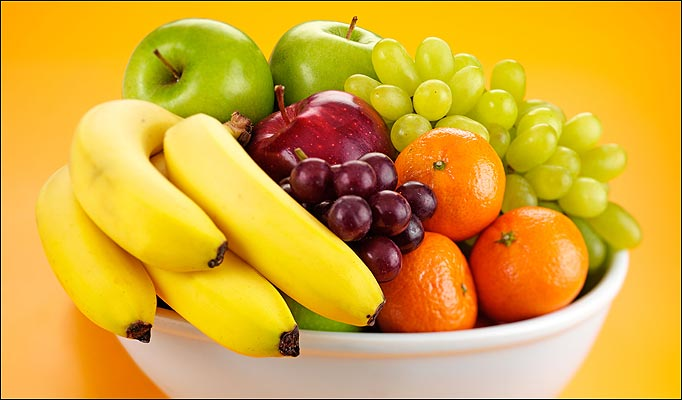
\includegraphics[scale=0.5]{fruitbowl2}
    \caption{Alternative Bowl of fruit}
    \label{fig:newFruit}
\end{figure}

\subsection*{Overview}
In our three previous sliding window oriented experiments, we had only used a
single image. In order to see whether this image had biases unknown
to us, I decided to use another fruit bowl image. This image was selected as
fruit took up a larger portion of the image as seen in Figure \ref{fig:newFruit}

\subsection*{Results}
\subsubsection*{Grid}
\subsubsection*{Row}
\subsubsection*{Column}

\subsection*{Analysis}
